\documentclass[12pt, a4paper, oneside]{ctexart}
\usepackage{amsmath, amsthm, amssymb, bm, color, graphicx, geometry, hyperref, mathrsfs,extarrows, braket, booktabs, array}

\linespread{1.4}
%\geometry{left=2.54cm,right=2.54cm,top=3.18cm,bottom=3.18cm}
\geometry{left=1.84cm,right=1.84cm,top=2.18cm,bottom=2.18cm}
\newenvironment{problem}{\par\noindent\textbf{题目. }}{\bigskip\par}
\newenvironment{solution}{\par\noindent\textbf{解答. }}{\bigskip\par}
\newenvironment{note}{\par\noindent\textbf{注记. }}{\bigskip\par}

\everymath{\displaystyle} % 默认全部行间公式
\DeclareMathOperator*\uplim{\overline{lim}} % 定义上极限 \uplim_{}
\DeclareMathOperator*\lowlim{\underline{lim}} % 定义下极限 \lowlim_{}
\let\leq=\leqslant % 将全部leq变为leqslant
\let\geq=\geqslant % geq同理

% 一些宏定义
\def\bd{\boldsymbol}    % 加粗(向量) boldsymbol
\def\disp{\displaystyle}% 使用行间公式 displaystyle(默认)
\def\tsty{\textstyle}   % 使用行内公式 textstyle
\def\sign{\text{sign}}  % sign function
\def\wtd{\widetilde}    % 宽波浪线 widetilde
\def\R{\mathbb{R}}      % Real number
\def\C{\mathbb{C}}      % Complex number
\def\d{\mathrm{d}}      % differential operator
\def\e{\mathrm{e}}      % Euler's number
\def\i{\mathrm{i}}      % imaginary number
\def\re{\mathrm{Re}}    % Real part
\def\im{\mathrm{Im}}    % Imaginary part
\def\L{\mathcal{L}}     % Loss function
\def\wdh{\widehat}      % 宽帽子 widehat
\def\ol{\overline}      % 上横线 overline
\def\ul{\underline}     % 下横线 underline
\def\add{\vspace{1ex}}  % 增加行间距
\def\del{\vspace{-3.5ex}}  % 减少行间距

% 基本信息
\newcommand{\RQ}{\today} % 日期
\newcommand{\km}{数值分析} % 科目
\newcommand{\bj}{强基数学002} % 班级
\newcommand{\xm}{吴天阳} % 姓名
\newcommand{\xh}{2204210460} % 学号
\newcommand{\XH}{59} % 序号

\begin{document}

%\pagestyle{empty}
\pagestyle{plain}
\vspace*{-15ex}
\centerline{\begin{tabular}{*6{c}}
    \parbox[t]{0.25\linewidth}{\begin{center}\textbf{日期}\\ \large \textcolor{blue}{\RQ}\end{center}} 
    & \parbox[t]{0.15\linewidth}{\begin{center}\textbf{科目}\\ \large \textcolor{blue}{\km}\end{center}}
    & \parbox[t]{0.2\linewidth}{\begin{center}\textbf{班级}\\ \large \textcolor{blue}{\bj}\end{center}}
    & \parbox[t]{0.1\linewidth}{\begin{center}\textbf{姓名}\\ \large \textcolor{blue}{\xm}\end{center}}
    & \parbox[t]{0.15\linewidth}{\begin{center}\textbf{学号}\\ \large \textcolor{blue}{\xh}\end{center}}
    & \parbox[t]{0.1\linewidth}{\begin{center}\textbf{序号}\\ \large \textcolor{blue}{\XH}\end{center}} \\ \hline
\end{tabular}}
\vspace*{4ex}

\paragraph{9.1}取$h=0.1$, 用欧拉法、后退欧拉法、中点法、梯形法求解初值问题:
\begin{equation*}
    y' = 1-y,\qquad y(0) = 0,\qquad 0\leq x\leq 1.
\end{equation*}
\begin{solution}
     欧拉法: $y_{i+1} = y_i+hf(x_i, y_i) = 0.9y_i+0.1$, 根据递推式可得
     \begin{equation*}
     \begin{array}{l}
        y_0 = 0.000,\quad y_1 = 0.100,\quad y_2 = 0.190,\quad y_3 = 0.271,\quad y_4 = 0.344,\quad y_5 = 0.410,\\
        y_6 = 0.469, \quad y_7 = 0.522, \quad y_8 = 0.570,\quad y_9 = 0.613,\quad y_{10} = 0.652.
     \end{array}
     \end{equation*}

     后退欧拉法: $y_{i+1} = y_i  +hf(x_{i+1}, y_{i+1})\Rightarrow y_{i+1} = \frac{10}{11}y_i+\frac{1}{11}$, 根据递推式可得
     \begin{equation*}
     \begin{array}{l}
        y_0 = 0.000,\quad y_1 = 0.091,\quad y_2 = 0.174,\quad y_3 = 0.249,\quad y_4 = 0.317,\quad y_5 = 0.379,\\
        y_6 = 0.435,\quad y_7 = 0.486,\quad y_8 = 0.533,\quad y_9 = 0.575,\quad y_{10} = 0.614.\\
     \end{array}
     \end{equation*}

     中点法: $y_{i+1} = y_{i-1}+2hf(x_i,y_i) = y_{i-1}-0.2y_i+0.2$, 根据线性微分方程解法, 原初值问题的解为$y = 1-e^{-x}$, 中点法的启动值取为$y_1 = 1-e^{-0.1}\approx 0.095$, 根据递推式可得
     \begin{equation*}
     \begin{array}{l}
         y_0 = 0.000,\quad y_1 = 0.095,\quad y_2 = 0.181,\quad y_3 = 0.259,\quad y_4 = 0.329,\quad y_5 = 0.393,\\
        y_6 = 0.450,\quad y_7 = 0.503,\quad y_8 = 0.549,\quad y_9 = 0.593,\quad y_{10} = 0.630.
     \end{array}
     \end{equation*}
     
     梯形法: $y_{i+1} = y_i+\frac{h}{2}(f(x_i,y_i)+f(x_{i+1},y_{i+1}))\Rightarrow y_{i+1}=\frac{2}{21}+\frac{19}{21}y_i$, 根据递推式可得
     \begin{equation*}
         \begin{array}{l}
            y_{0} = 0.000,\quad y_{1} = 0.095,\quad y_{2} = 0.181,\quad y_{3} = 0.259,\quad y_{4} = 0.330,\quad y_{5} = 0.394,\\
            y_{6} = 0.452,\quad y_{7} = 0.504,\quad y_{8} = 0.551,\quad y_{9} = 0.594,\quad y_{10} = 0.633.
         \end{array}
     \end{equation*}
\end{solution}\del
\paragraph{9.5}利用标准的$4$级$4$阶R-K法求解习题9.1.
\begin{solution}
    经典$4$级$4$阶R-K法递推式为
    \begin{equation*}
        \begin{cases}
            y_{i+1} = y_i+\frac{1}{6}(K_1+2K_2+2K_3+K_4),\\
            K_1 = hf(x_i, y_i),\\
            K_2 = hf\left(x_i+\frac{1}{2}h, y_i+\frac{1}{2}K_1\right),\add\\
            K_3 = hf\left(x_i+\frac{1}{2}h, y_i+\frac{1}{2}K_2\right),\\
            K_4 = hf(x_i+h, y_i+K_3).
        \end{cases}\Rightarrow\begin{cases}
            y_{i+1} = y_i+\frac{1}{6}(K_1+2K_2+2K_3+K_4),\\
            K_1 = -0.1y_i+0.1,\\
            K_2 = 0.1-0.1(y_i+0.5K_1),\\
            K_3 = 0.1-0.1(y_i+0.5K_2),\\
            K_4 = 0.1-0.1(y_i+K_3).
        \end{cases}
    \end{equation*}
    根据递推式可得
    \begin{equation*}
        \begin{array}{l}
            y_{0} = 0.000,\quad y_{1} = 0.095,\quad y_{2} = 0.181,\quad y_{3} = 0.259,\quad y_{4} = 0.330,\quad y_{5} = 0.394,\\
            y_{6} = 0.452,\quad y_{7} = 0.504,\quad y_{8} = 0.551,\quad y_{9} = 0.594,\quad y_{10} = 0.633.
        \end{array}
    \end{equation*}
\end{solution}
\paragraph{9.7}利用待定系数法确定以下求解公式中的系数, 使其阶数尽可能高, 并导出截断误差表达式:
\begin{equation*}
    y_{i+1} = \alpha_0 y_i+\alpha_1 y_{i-1}+\beta hf_{i+1}.
\end{equation*}
\begin{solution}
    由题可知, 截断误差为
    \begin{align*}
        R[y] = y(x_{i+1}) - y_{i+1} =&\ y(x_{i+1}) - \alpha_0 y(x_i)-\alpha_1y(x_{i-1}) - \beta hy'(x_{i+1})\\
        =&\ y(x_i+h)-\alpha_0y(x_i)-\alpha_1y(x_i-h)-\beta hy'(x_i+h),
    \end{align*}
    取$x_i=0$, 令$R[x^k] = 0\ (k=0,1,2)$得
    \begin{equation*}
        \begin{cases}
            1-\alpha_0-\alpha_1 = 0,\\
            h(1+\alpha_1-\beta) = 0,\\
            h^2(1-\alpha_1-2\beta) = 0.
        \end{cases}\Rightarrow\quad\begin{cases}
            \alpha_0 = \frac{4}{3},\\
            \alpha_1 = -\frac{1}{3},\\
            \beta = \frac{2}{3}.
        \end{cases}
    \end{equation*}
    则$y_{i+1} = \frac{1}{3}(4y_i-y_{i-1}+2hf_{i+1})$, 于是$R[y] = y(x_i+h) - \frac{4}{3}y(x_i)+\frac{1}{3}y(x_i-h)-\frac{2}{3}hy'(x_i+h)$, 取$x_i = 0$, 令$y = x^3$, 则
    \begin{equation*}
        R[x^3] = h^3-\frac{1}{h^3}-2h^3 = -\frac{4}{3}h^3\neq 0,
    \end{equation*}
    所以该公式的代数精度$m=2$, 取$e(x) = \frac{1}{3!}y^{(3)}(\xi)(x-x_{i+1})(x-x_i)(x-x_{i-1})$, 由广义Peano定理知, 截断误差表示式为
    \begin{equation*}
        R[y] = R[e(x)] = -\frac{2}{3}h\cdot \frac{1}{3!}y^3(\xi)(x_{i+1}-x_i)(x_{i+1}-x_{i-1}) = -\frac{2}{9}h^3y^3(\xi).
    \end{equation*}
\end{solution}\del\del
\paragraph{9.11}将以下高阶微分方程化为一阶微分方程组初值问题:
\begin{equation*}
    \begin{cases}
        y'' = y'(1-y^2)-y,\\
        y(x_0)=y_0,\ y'(x_0)=y_0'.
    \end{cases}
\end{equation*}
\begin{solution}
    令$y_1 = y,\ y_2 = y'$, 则原高阶方程等价于求解以下一阶微分方程组
    \begin{equation*}
        \begin{cases}
            y_1' = y_2,\\
            y_2' = y_2(1-y_1^2) - y_1,\\
            y_1(x_0) = y_0,\ y_2(x_0) = y_0'.
        \end{cases}
    \end{equation*}
\end{solution}
\iffalse
% 图片模板
\centerline{
    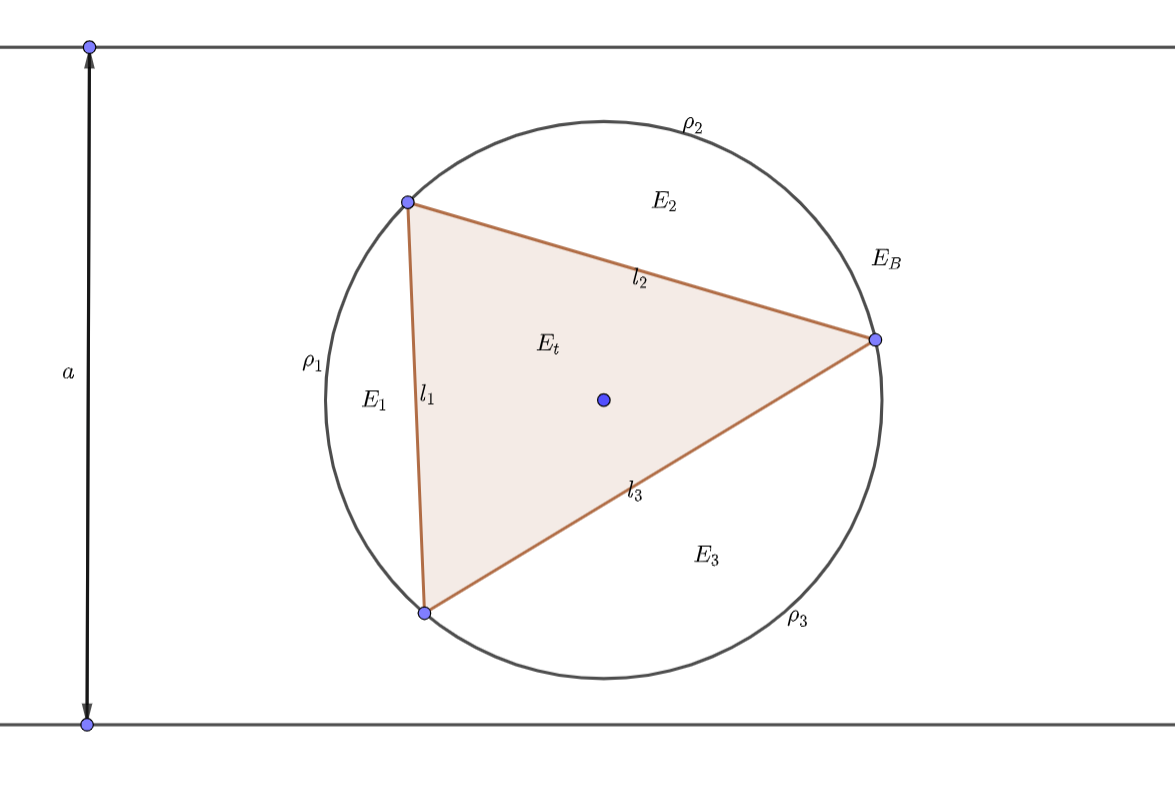
\includegraphics[width=0.8\textwidth]{figure.png}
}
\fi
\iffalse
% 表格模板
\renewcommand\arraystretch{0.8} % 设置表格高度为原来的0.8倍
\begin{table}[!htbp] % table标准
    \centering % 表格居中
    \begin{tabular}{p{1cm}<{\centering}p{1cm}<{\centering}p{3cm}<{\centering}p{5cm}<{\centering}} % 设置表格宽度
    %\begin{tabular}{cccc}
        \toprule
        $x_i$ & $f[x_1]$ & $f[x_i,x_{i+1}]$ & $f[x_i,x_{i+1},x_{i+2}]$ \\
        \midrule
        $x_0$ & $f(x_0)$ &                  &                          \\
        $x_0$ & $f(x_0)$ & $f'(x_0)$        &                          \\
        $x_0$ & $f(x_1)$ & $\frac{f(x_1)-f(x_0)}{x_1-x_0}$ & $\frac{f(x_1)-f(x_0)}{(x_1-x_0)^2}-\frac{f'(x_0)}{x_1-x_0}$\\
        \bottomrule
    \end{tabular}
\end{table}

\def\Log{\text{Log}} % 一个简单的宏定义
$\Log$ % 调用方法
\fi

\end{document}